\documentclass[a4paper, 11pt]{article}
\usepackage[pdftex]{graphicx}
\usepackage{fullpage}
\usepackage{mathrsfs,amsmath}


% An example of defining macros
\newcommand{\rs}[1]{\mathstrut\mbox{\scriptsize\rm #1}}
\newcommand{\rr}[1]{\mbox{\rm #1}}
% My equations
%-----------------------------------------------------------
\renewcommand{\div}{\nabla\cdot}
\newcommand{\grad}{\vec \nabla}
\newcommand{\curl}{{\vec \nabla}\times}
\renewcommand{\H}{{\vec H}}
\newcommand {\J}{{\vec J}}
\newcommand {\E}{{\vec E}}
\newcommand{\siginf}{\sigma_\infty}
\newcommand{\dsig}{\triangle\sigma}
\newcommand{\dcurl}{{\mathbf C}}
\newcommand{\dgrad}{{\mathbf G}}
\newcommand{\Acf}{{\mathbf A_c^f}}
\newcommand{\Ace}{{\mathbf A_c^e}}
\renewcommand{\S}{{\mathbf \Sigma}}
\newcommand{\St}{{\mathbf \Sigma_\tau}}
\newcommand{\T}{{\mathbf T}}
\newcommand{\Tt}{{\mathbf T_\tau}}
\newcommand{\diag}{\mathbf{diag}}
\newcommand{\M}{{\mathbf M}}
\newcommand{\MfMui}{{\M^f_{\mu^{-1}}}}
\newcommand{\MfMuoi}{{\M^f_{\mu_0^{-1}}}}
\newcommand{\dMfMuI}{{d_m (\M^f_{\mu^{-1}})^{-1}}}
\newcommand{\dMfMuoI}{{d_m (\M^f_{\mu_0^{-1}})^{-1}}}
\newcommand{\MeSig}{{\M^e_\sigma}}
\newcommand{\MeSigInf}{{\M^e_{\sigma_\infty}}}
\newcommand{\MeSigInfEtab}{{\M^e_{\sigma_\infty \bar{\eta}}}}
\newcommand{\MeSigInfEtat}{{\M^e_{\sigma_\infty \peta}}}
\newcommand{\MedSig}{{\M^e_{\triangle\sigma}}}
\newcommand{\MeSigO}{{\M^e_{\sigma_0}}}
\newcommand{\Me}{{\M^e}}
\newcommand{\Js}{\mathbf{J}^s}
\newcommand{\Mes}[1]{{\M^e_{#1}}}
\newcommand{\Mee}{{\M^e_e}}
\newcommand{\Mej}{{\M^e_j}}
\newcommand{\BigO}[1]{\mathcal{O}\bigl(#1\bigr)}
\newcommand{\bE}{\mathbf{E}}
\newcommand{\bEp}{\mathbf{E}^p}
\newcommand{\bB}{\mathbf{B}}
\newcommand{\bBp}{\mathbf{B}^p}
\newcommand{\bEs}{\mathbf{E}^s}
\newcommand{\bBs}{\mathbf{B}^s}
\newcommand{\bH}{\mathbf{H}}
\newcommand{\B}{\vec{B}}
\newcommand{\D}{\vec{D}}
\renewcommand{\H}{\vec{H}}
\newcommand{\s}{\vec{s}}
\newcommand{\bfJ}{\bf{J}}
\newcommand{\vecm}{\vec m}
\renewcommand{\Re}{\mathsf{Re}}
\renewcommand{\Im}{\mathsf{Im}}
\renewcommand {\j}  { {\vec j} }
\newcommand {\h}  { {\vec h} }
\renewcommand {\b}  { {\vec b} }
\newcommand {\e}  { {\vec e} }
\renewcommand {\d}  { {\vec d} }
\renewcommand {\u}  { {\vec u} }

\renewcommand {\dj}  { {\mathbf{j} } }
\renewcommand {\dh}  { {\mathbf{h} } }
\newcommand {\db}  { {\mathbf{b} } }
\newcommand {\de}  { {\mathbf{e} } }

\newcommand{\vol}{\mathbf{v}}
\newcommand{\I}{\vec{I}}
\newcommand{\A}{\mathbf{A}}
\newcommand{\bI}{\mathbf{I}}
\newcommand{\bus}{\mathbf{u}^s}
\newcommand{\brhss}{\mathbf{rhs}_s}
\newcommand{\bup}{\mathbf{u}^p}
\newcommand{\brhs}{\mathbf{rhs}}
%%-------------------------------
\newcommand{\bon}{b^{on}(t)}
\newcommand{\bp}{b^{p}}
\newcommand{\dbondt}{\frac{db^{on}(t)}{dt}}
\newcommand{\dfdt}{\frac{df(t)}{dt}}
\newcommand{\dbdt}{\frac{\partial \b}{\partial t}}
\newcommand{\dfdtdsiginf}{\frac{\partial\frac{df(t)}{dt}}{\partial\siginf}}
\newcommand{\dfdsiginf}{\frac{\partial f(t)}{\partial\siginf}}
\newcommand{\dbgdsiginf}{\frac{\partial b^{Impulse}(t)}{\partial\siginf}}
\newcommand{\digint}{\frac{2}{\pi}\int_0^{\infty}}
\newcommand{\Gbiot}{\mathbf{G}_{Biot}}
%%-------------------------------
\newcommand{\peta}{\tilde{\eta}}
\newcommand{\petadt}{\frac{\partial \tilde{\eta}}{\partial t}}
\newcommand{\eFmax}{\e^{F}_{max}}
\newcommand{\dip}{d^{IP}}
\newcommand{\sigpert}{\delta\sigma}


\newcommand{\SimPEG}{\textsc{SimPEG}\xspace}
\newcommand{\simpegEM}{\textsc{simpegEM}\xspace}


\begin{document}
\graphicspath{{./IPFigures/}}


\section{IP sphere}

%%%%%%%%%%%%%%%%%%%%%%%%%%%%%%%%%%%%%%%%%%%%%%%%%%%%%%%%%%%%%%%%%%%%%%%%%%%%%
%%%%%%%%%%%%%%%%%%%%%%%%%%%%%%%%%%%%%%%%%%%%%%%%%%%%%%%%%%%%%%%%%%%%%%%%%%%%%

\subsection{Electric fields}
In order to get some insights of IP responses, we apply complex conductivity model to the static sphere problem.
Here we can plug in complex conductivity model to $\sigma_2$. Assume that we know solutions of electric fields for a conductive sphere of radius $R$ in a uniform electrostatic case: \\
The electric field outside ($r>R$) is 
\begin{equation}
	\E_1 = E_0\hat{x}+E_0R^3\frac{\sigma_2(\omega)-\sigma_1}{\sigma_2(\omega)+2\sigma_1}\frac{(2x^2-y^2-z^2)\hat{x}+(3xy)\hat{y}+(3xz)\hat{z}}{r^5},
\label{eq:IPspheq1}		
\end{equation}
and inside ($r<R$) is
\begin{equation}
	\E_2 = E_0\frac{3\sigma_1}{\sigma_2(\omega)+2\sigma_1}\hat{x},
\label{eq:IPspheq2}		
\end{equation}
where 
\begin{displaymath}
	\sigma_2(\omega) = \siginf(1-\frac{\eta}{1+(1-\eta)(\imath\omega\tau)^c}).
\end{displaymath}
Without any IP effect, electric field and current for three different cases are shown in Figure \ref{fig:DCEJFund}. Classification of the models are $^{1)}$ Conductive ($\sigma_2 > \sigma_1$) $^{2)}$ Resistive ($\sigma_2 > \sigma_1$) and $^{3)}$ Canonical ($\sigma_2 = \sigma_1$). 

\begin{figure}[htb]
  \centering
  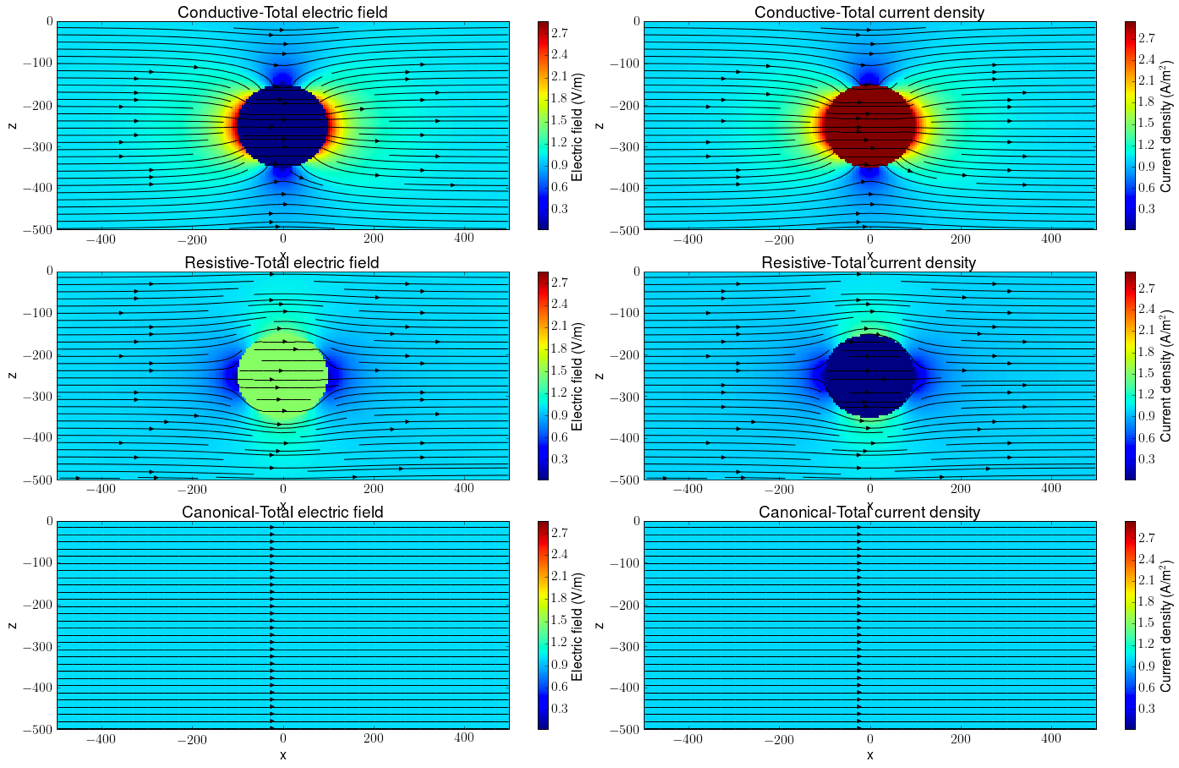
\includegraphics[width=1.0\textwidth]{DCEJFund.png}
  \caption{Electric field and current density sections of three different models: $^{1)}$ Conductive ($\sigma_2 > \sigma_1$) $^{2)}$ Resistive ($\sigma_2 > \sigma_1$) and $^{3)}$ Canonical ($\sigma_2 = \sigma_1$). $\sigma_1$ is 1 S/m and $\sigma_1 / \sigma_2$ for conductive and resistive cases are set to 10$^{2}$and 10$^{-2}$, respectively. }
  \label{fig:DCEJFund}
\end{figure}

To make our problem simple, we use $c=1$. Then we have
\begin{displaymath}
	\sigma_2(\omega) = \siginf(1-\frac{\eta}{1+(1-\eta)(\imath\omega\tau)}).
\end{displaymath}
Since we are using the time dependency, $e^{-\imath\omega t}$, we use $\sigma_2(\omega)^*$. If you think about time domain responses of equations~\ref{eq:IPspheq1} and ~\ref{eq:IPspheq2}, they are only dependent of $\sigma_2(\omega)$; thus, we substitute some related variables:
\begin{align*}
	\E_1 = E_0\hat{x}+k_1(\omega)E_0R^3\frac{(2x^2-y^2-z^2)\hat{x}+(3xy)\hat{y}+(3xz)\hat{z}}{r^5}\\
	=E_0\hat{x}+k_1(\omega)\vec{P} \\
	\E_2 = E_0k_2(\omega)\hat{x},\\
	k_1(\omega)=\frac{\sigma_2^*(\omega)-\sigma_1}{\sigma_2(\omega)^*+2\sigma_1},\\
	k_2(\omega)=\frac{3\sigma_1}{\sigma_2(\omega)^*+2\sigma_1}.\\
	\vec{P} = E_0R^3\frac{(2x^2-y^2-z^2)\hat{x}+(3xy)\hat{y}+(3xz)\hat{z}}{r^5}
\end{align*}
We calculate step-off responses of these by using inverse Fourier transform:
\begin{align*}
	\e(t) = \frac{1}{2\pi}\int_{-\infty}^{\infty}\frac{\E(\omega)}{\imath\omega}e^{-\imath\omega t} d\omega.
\end{align*}
The electric field out- and inside are
\begin{align*}
	\e_1(t) = E_0u(-t)\hat{x} + k_1(t)\vec{P}, \\
	\e_2(t) = k_2(t)E_0\hat{x},
\end{align*}
where
\begin{align*}
	k_1(t) = \frac{1}{2\pi}\int_{-\infty}^{\infty}\frac{k_1(\omega)}{\imath\omega}e^{-\imath\omega t} d\omega, \\
	k_2(t) = \frac{1}{2\pi}\int_{-\infty}^{\infty}\frac{k_2(\omega)}{\imath\omega}e^{-\imath\omega t} d\omega.
\end{align*}

\begin{equation*}
	k_1(t) = \frac{\siginf(1-\eta)-\sigma_1}{\siginf(1-\eta)+2\sigma_1}u(-t)
	- \frac{3\sigma_1\siginf\eta}{(\siginf+2\sigma_1)(\siginf(1-\eta)+2\sigma_1)})
	e^{-\frac{(\siginf(1-\eta)+2\sigma_1)}{(\siginf + 2\sigma_1)((1-\eta)\tau)}t}
\end{equation*}
\begin{equation*}
	k_2(t) = \frac{3\sigma_1}{\siginf(1-\eta)+2\sigma_1}u(-t)
	- \frac{3\sigma_1\siginf\eta}{(\siginf+2\sigma_1)(\siginf(1-\eta)+2\sigma_1)})
	e^{-\frac{(\siginf(1-\eta)+2\sigma_1)}{(\siginf + 2\sigma_1)((1-\eta)\tau)}t}
\end{equation*}

\begin{align*}
	\e_1(t) = u(-t)(E_0\hat{x}+\frac{\siginf(1-\eta)-\sigma_1}{\siginf(1-\eta)+2\sigma_1} \vec{P})  - \frac{3\sigma_1\siginf\eta}{(\siginf+2\sigma_1)(\siginf(1-\eta)+2\sigma_1)})
	e^{-\frac{(\siginf(1-\eta)+2\sigma_1)}{(\siginf + 2\sigma_1)((1-\eta)\tau)}t}\vec{P}, \\
	\e_2(t) = \frac{3\sigma_1}{\siginf(1-\eta)+2\sigma_1}u(-t)E_0\hat{x}
	+ \frac{3\sigma_1\siginf\eta}{(\siginf+2\sigma_1)(\siginf(1-\eta)+2\sigma_1)})
	e^{-\frac{(\siginf(1-\eta)+2\sigma_1)}{(\siginf + 2\sigma_1)((1-\eta)\tau)}t}E_0\hat{x}
\end{align*}
By letting 
\begin{eqnarray*}
	\bar{R}_1 = \frac{\sigma_2 (1-\eta)-\sigma_1}{\sigma_2(1-\eta) + 2\sigma_1} \\
	\bar{R}^{\sigma_2}_1 = \frac{\sigma_2 \eta}{\sigma_2(1-\eta) + 2\sigma_1} \\
	R_1 = \frac{\sigma_2-\sigma_1}{\sigma_2 + 2\sigma_1} \\
	\bar{R}_2 = \frac{3\sigma_1}{\sigma_2(1-\eta) + 2\sigma_1} \\
	R_2 = \frac{3\sigma_1}{\sigma_2 + 2\sigma_1} \\
	A = R_2\bar{R}^{\sigma_2}_1 \\
	B = \frac{\sigma_2(1-\eta)+2\sigma_1}{\sigma_2 + 2\sigma_1}b \\
	b = \frac{1}{(1-\eta)\tau} \\
	a = \frac{\eta}{(1-\eta)\tau} \\
	\sigma_2 = \siginf
	\E^p = E_0\hat{x}
\end{eqnarray*}
we have
\begin{align*}
	\e_1(t) = u(-t)(\E^p+\bar{R}_1 \vec{P})  - A
	e^{-Bt}\vec{P}, \\
	\e_2(t) = \bar{R}_2u(-t)\E^p
	- Ae^{-Bt}\E^p,
\end{align*}
At off time response, amplitude of IP response proportional to $A$. 
\begin{align*}
	A = \frac{3\sigma_1}{\sigma_2 + 2\sigma_1} \frac{\sigma_2 \eta}{\sigma_2(1-\eta) + 2\sigma_1} \\
	= \frac{3\sigma_1 / \sigma_2}{ 1+ 2 \sigma_1 / \sigma_2} 
	\frac{\eta}{(1-\eta) + 2\sigma_1/ \sigma_2}
\end{align*}
Limit values of $A$ are 
\begin{align}
	\lim_{ \sigma_1/ \sigma_2 \to\infty} A = 0 \\
	\lim_{ \sigma_1/ \sigma_2 \to 0} A = 0 \\
	\lim_{ \sigma_1/ \sigma_2 \to 1} A = \frac{\eta}{3-\eta} 
\end{align}
This shows the IP response has maximum not when we have perfect conductor, but when we have canonical model, which does not have any conductivity contrast. This is an interesting result, which I do not have a good physical reasoning behind. 
The term $B$ shows how IP response decays. Limit values of $B$ are 
\begin{align}
	\lim_{ \sigma_1/ \sigma_2 \to\infty} B = -b = \frac{1}{(1-\eta)\tau}\\
	\lim_{ \sigma_1/ \sigma_2 \to0} B = \frac{1}{\tau} \\
	\lim_{ \sigma_1/ \sigma_2 \to1} B = \frac{3-\eta}{3}\frac{1}{(1-\eta)\tau}
\end{align}

In order to realize IP response from general waveform, we need to compute impulse response. By taking the derivative of $\e(t)$ $w.r.t$ time, we obtain impulse response:
\begin{equation*}
	\e^{ \ Impulse} = -\frac{\partial \e^{\ off}}{\partial t }
\end{equation*}
\begin{align*}
	\e^{\ off}_1(t) = u(-t)(\E^p+\bar{R}_1 \vec{P})  - Ae^{-Bt}\vec{P}u(t)
\end{align*}
\begin{equation*}
	\e^{ \ Impulse}_1 =  \delta(t)(\E^p+(\bar{R}_1+A) \vec{P})  +-\frac{A}{B}e^{-Bt}\vec{P}u(t)
\end{equation*}
\begin{equation*}
	\e^{ \ general}_1(t) =  \e^{ \ Impulse}_1(t) \otimes w(t),
\end{equation*}
where $w(t)$ is a general transmitter waveform. 
%%%%%%%%%%%%%%%%%%%%%%%%%%%%%%%%%%%%%%%%%%%%%%%%%%%%%%%%%%%%%%%%%%%%%%%%%%%%%
%%%%%%%%%%%%%%%%%%%%%%%%%%%%%%%%%%%%%%%%%%%%%%%%%%%%%%%%%%%%%%%%%%%%%%%%%%%%%

\subsection{Currents}
Using Ohm's law current density can be expressed as 
\begin{equation}
	\j(t) = \sigma(t) \otimes \e(t).
\end{equation}
By the definition of $\sigma(t)$ ($=\siginf\delta(t) + \dsig(t)$) we have
\begin{equation}
	\j(t) = \siginf\e(t) + \dsig(t)\otimes \e(t).
\end{equation}
Inside of the body, we have
\begin{align*}
	\e_2(t) = \bar{R}_2u(-t)\E^p
	- Ae^{-Bt}\E^p
\end{align*}
\begin{equation}
	\j_2(t) = \siginf\e_2(t) = \sigma_2 \e(t) = \sigma_2\bar{R}_2 u(-t)\E^{p} + ^{(a)} \sigma_2 A e^{-Bt}\E^{p},
\end{equation}
\begin{equation}
	\dsig(t)\otimes \e_2(t) =  - ^{(b)} \sigma_2 \bar{R}_2\eta e^{-bt}\E^{p} - ^{(c)} \sigma_2 A\frac{a}{b-B}(e^{(b-B)t}-1)e^{-bt}\E^{p}.
\end{equation}
Outside of the body we have
\begin{align*}
	\e_1(t) = u(-t)(\E^p+\bar{R}_1 \vec{P})  - A
	e^{-Bt}\vec{P}
\end{align*}
\begin{equation}
	\j_1(t) = \siginf\e_1(t) = \sigma_1 \e(t) = \sigma_1(\E^p+\bar{R}_1 \vec{P}) - \sigma_1 A e^{-Bt}\vec{P},
\end{equation}
Using $\siginf$ as a reference conductivity, we can decompose electric field as 
\begin{equation*}
	\e = \e^{F} + \e^{IP}
\end{equation*}
Then IP current can be expressed as we have
\begin{equation*}
	\j^{IP} = \siginf\e^{IP} + \dsig(t)\otimes\e^{F} + \dsig(t)\otimes\e^{IP}
\end{equation*}
The first term is same as $(a)$. However, the second and third terms are not same as $(b)$ and $(c)$. Inside of the body, 
\begin{equation*}
	\j^{IP}_1 = \siginf\e^{IP}
\end{equation*}
\begin{equation*}
	\j^{IP}_2 = \dsig(t)\otimes\e^{F} = - \sigma_2 (\bar{R}_2-A)\eta e^{-bt}\E^{p}.
\end{equation*}
\begin{equation*}
	\j^{IP}_3 = \dsig(t)\otimes\e^{IP} = +\sigma_2 (A)\eta e^{-bt}\E^{p} - \sigma_2 A\frac{a}{b-B}(e^{(b-B)t}-1)e^{-bt}\E^{p}.
\end{equation*}
Relative strength fo each term are shown in Figure  \ref{fig:jipcurves}.

\begin{figure}[htb]
  \centering
  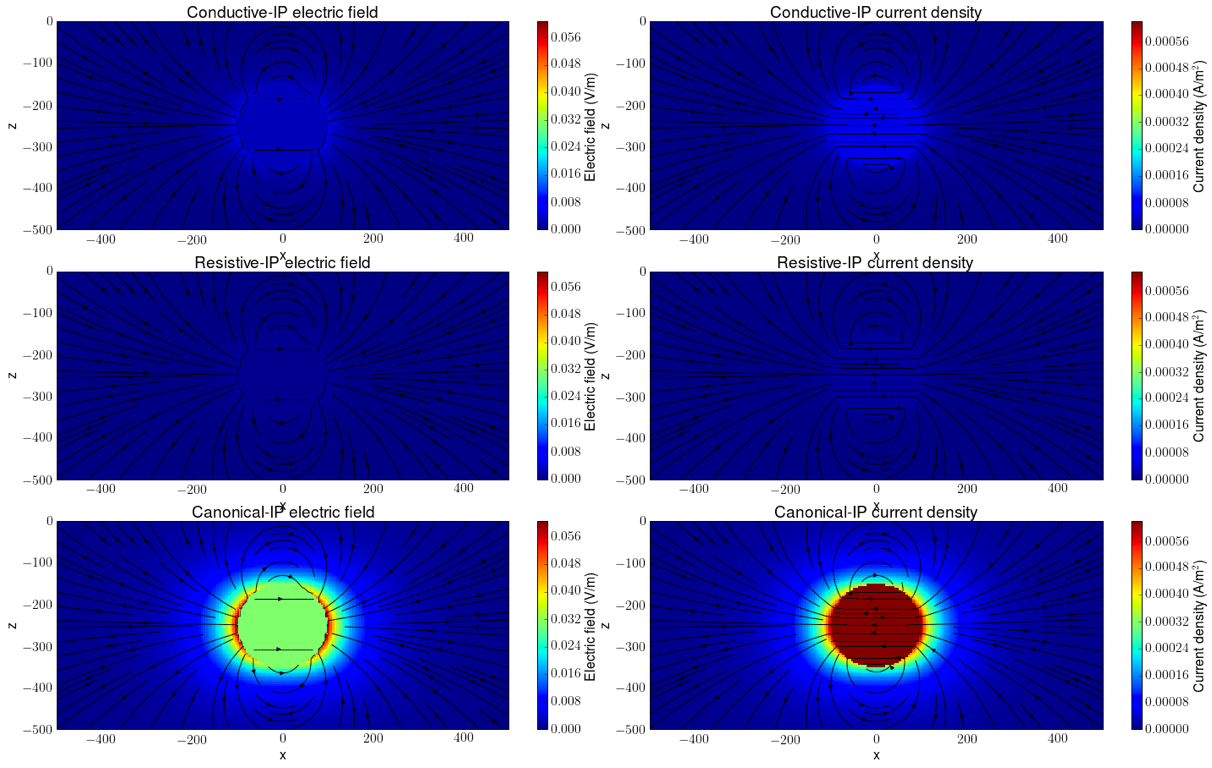
\includegraphics[width=1.0\textwidth]{DCEJIP.png}
  \caption{Electric field and current density sections of three different models: $^{1)}$ Conductive ($\sigma_2 > \sigma_1$) $^{2)}$ Resistive ($\sigma_2 > \sigma_1$) and $^{3)}$ Canonical ($\sigma_2 = \sigma_1$). $\sigma_1$ is 1 S/m and $\sigma_1 / \sigma_2$ for conductive and resistive cases are set to 10$^{2}$and 10$^{-2}$, respectively. }
  \label{fig:DCEJIP}
\end{figure}

\begin{figure}[htb]
  \centering
  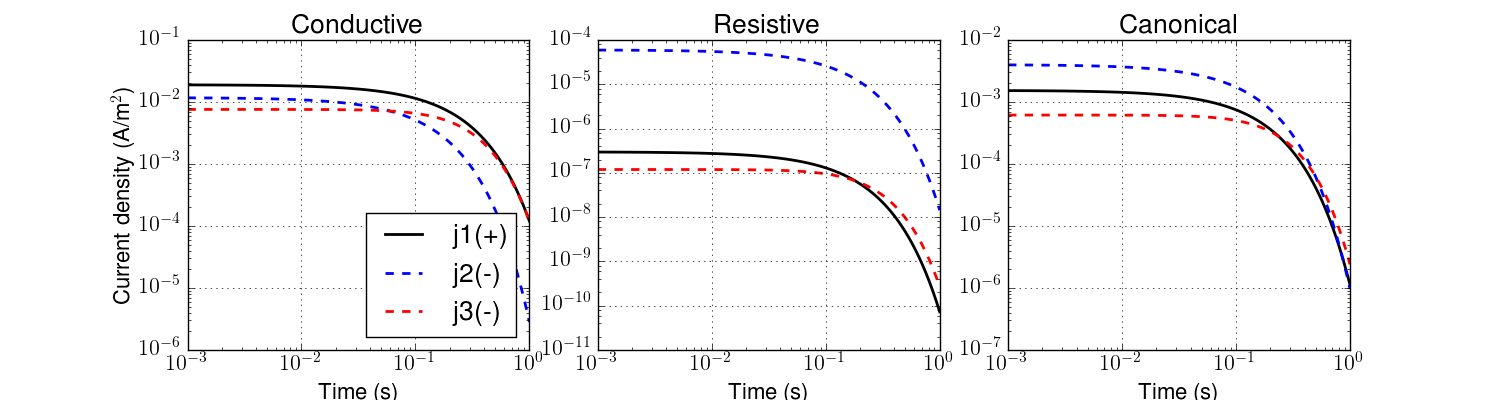
\includegraphics[width=1.0\textwidth]{jipcurves.png}
  \caption{Comparison of IP currents in the IP body. $\sigma_1$ is fixed to 10$^{-1}$, and $\sigma_2$ are 10$^{-1}$, 10$^{-5}$, 10$^{-3}$ for corresponding cases.$\eta$ and $\tau$ are 0.4 and 0.2, respectively.}
  \label{fig:jipcurves}
\end{figure}

\clearpage

\end{document}
